\documentclass[preview]{standalone}
\usepackage{tikz}
\usepackage{mathptmx}
\usepackage{avant}
\renewcommand*\familydefault{\sfdefault}
\usepackage[T1]{fontenc}
\usetikzlibrary{positioning, backgrounds, shapes, chains, arrows, decorations.pathmorphing, matrix, fit}


\begin{document}

%\vspace{0.1cm}

  \begin{center}
    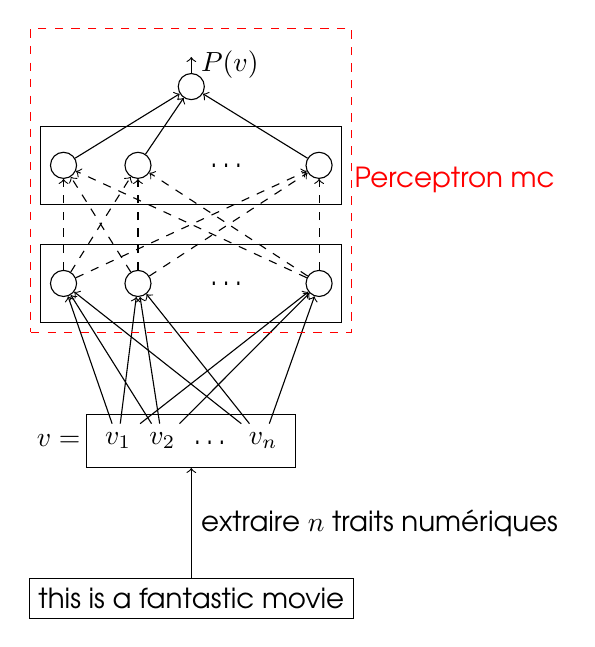
\begin{tikzpicture}
      \begin{scope}[ampersand replacement=\&]
        \matrix (v) [draw, every node/.style={outer sep=0}, matrix of nodes, nodes in empty cells, execute at empty cell=\node{\strut}] at (0, 2){
        $v_1$ \& $v_2$ \& \dots \& $v_n$\\
        };
        \matrix (l1) [draw, column sep=0.6cm, matrix of nodes, nodes in empty cells, nodes={circle, draw, anchor=center, align=center}] at (0, 4){
         \& \& |[draw=none]| \dots \& \\
        };
        \matrix (l2) [draw, column sep=0.6cm, matrix of nodes, nodes in empty cells, nodes={circle, draw, anchor=center, align=center}] at (0, 5.5){
         \& \& |[draw=none]| \dots \& \\
        };
        \node[circle, draw] (out) at (0, 6.5) {};
        \node (end) at (0, 7) {};
      \end{scope}
      \node[xshift=-3mm] (vname) at (v.west) {$v = {}$};
      \node[rectangle, draw] (text) at (0, 0) {this is a fantastic movie};
      \path (text) edge[->] node[midway, right]{extraire $n$ traits num\'eriques} (v);
      \path (v-1-1) edge[->] (l1-1-1);
      \path (v-1-1) edge[->] (l1-1-2);
      \path (v-1-1) edge[->] (l1-1-4);
      \path (v-1-2) edge[->] (l1-1-1);
      \path (v-1-2) edge[->] (l1-1-2);
      \path (v-1-2) edge[->] (l1-1-4);
      \path (v-1-4) edge[->] (l1-1-1);
      \path (v-1-4) edge[->] (l1-1-2);
      \path (v-1-4) edge[->] (l1-1-4);

      \path (l1-1-1) edge[dashed, ->] (l2-1-1);
      \path (l1-1-1) edge[dashed, ->] (l2-1-2);
      \path (l1-1-1) edge[dashed, ->] (l2-1-4);
      \path (l1-1-2) edge[dashed, ->] (l2-1-1);
      \path (l1-1-2) edge[dashed, ->] (l2-1-2);
      \path (l1-1-2) edge[dashed, ->] (l2-1-4);
      \path (l1-1-4) edge[dashed, ->] (l2-1-1);
      \path (l1-1-4) edge[dashed, ->] (l2-1-2);
      \path (l1-1-4) edge[dashed, ->] (l2-1-4);

      \path (l2-1-1) edge[->] (out);
      \path (l2-1-2) edge[->] (out);
      \path (l2-1-4) edge[->] (out);

      \path (out) edge[->] node[midway, right] {$P(v)$} (end);

      \node[draw, rectangle, color=red, dashed, fit=(end.north) (l1.south) (l1.west) (l1.east)] (mlp) {};
      \node[color=red, xshift=13mm] at (mlp.east) {Perceptron mc};
    \end{tikzpicture}
  \end{center}
  
  \vspace{0.1cm}
\end{document}
